\documentclass{article}
\usepackage[UTF8]{ctex}
\usepackage{amsmath}
\usepackage{amssymb}
\usepackage{tikz}
\usepackage{xcolor}
\usetikzlibrary{arrows,shapes,chains}
\usepackage{cite}
\usepackage{graphicx}
\usepackage{subfigure}
\usepackage{listings}
\usepackage{float}
%\usepackage[framed,numbered,autolinebreaks,useliterate]{mcode}

\title{Code1 实验报告}
\author{郑涛 SA24001077}
\date{\today}

\begin{document}
	\maketitle
	\section{问题描述}
	本次实验目的是实现一维多项式插值和RBF插值,实现了不同$b_0$的RBF并进行比较。
	\section{程序思路说明}
	给定插值点$p_i(x_i,y_i)$
	\subsection{多项式插值}
	多项式插值基函数为$x^i(i=0,1,2,\cdots,n-1)$,插值函数为
	$$f(x)=\sum_{i=0}^{n-1}w_ix^i$$
	其中$w_i$为基函数权重,可以根据求解下列方程组得到:
	\begin{equation}
		\left[
		\begin{array}{ccccc}
			1      & x_1    & x_1^2 & \cdots&x_1^{n-1}\\
			1      & x_2    & x_2^2 & \cdots&x_2^{n-1}\\
			\vdots & \vdots & \cdots& \vdots&\cdots\\
			1      & x_n    & x_n^2 & \cdots&x_n^{n-1}
		\end{array}
		\right]
		\left[
		\begin{array}{c}
			w_1     \\
			w_2     \\
			\vdots\\
			w_n     
		\end{array}
		\right]
		=
		\left[
		\begin{array}{c}
			y_1     \\
			y_2     \\
			\vdots\\
			y_n     
		\end{array}
		\right]
	\end{equation}
\subsection{RBF插值}
	RBF插值基函数为径向基函数:
$$g_{i}(x)=\frac{1}{|x-p_{i}|^2+d}$$
RBF插值函数为:
	$$f(x)=b_0+\sum_{i=1}^{n}b_{i}g_{i}(x)$$
	其中$b_i(i=0,1,\cdots,b_n)$均为常系数,可以根据如下方程组求解得到:
	\begin{equation}
		\left[
		\begin{array}{ccccc}
			g_1(x_1)      & g_1(x_2)    & g_1(x_3) & \cdots&g_1(x_n)\\
			g_2(x_1)      & g_2(x_2)    &g_2(x_3) & \cdots&g_2(x_n)\\
			\vdots & \vdots & \cdots& \vdots&\cdots\\
			g_n(x_1)      & g_n(x_2)    & g_n(x_3) & \cdots&g_n(x_n)
		\end{array}
		\right]
		\left[
		\begin{array}{c}
			b_1     \\
			b_2     \\
			\vdots\\
			b_n     
		\end{array}
		\right]
		=
		\left[
		\begin{array}{c}
			y_1-b_0     \\
			y_2-b_0     \\
			\vdots\\
			y_n-b_0     
		\end{array}
		\right]
	\end{equation}
其中$b_0$也可以用低阶多项式$b_0(x)$代替,如用k阶多项式代替,$b_0$为k阶多项式的近似函数$b_0(x)=\sum_{i=0}^{k}c_ix^i$,系数$c_i$由下列方程组给出
\begin{equation}
	\left[
	\begin{array}{ccccc}
			1      & x_1    & x_1^2 & \cdots&x_1^k\\
		1      & x_2    & x_2^2 & \cdots&x_2^k\\
		\vdots & \vdots & \cdots& \vdots&\cdots\\
		1      & x_n    & x_n^2 & \cdots&x_n^k
	\end{array}
	\right]
	\left[
	\begin{array}{c}
		c_0     \\
		c_1     \\
		\vdots\\
		c_k     
	\end{array}
	\right]
	=
	\left[
	\begin{array}{c}
		y_1     \\
		y_2     \\
		\vdots\\
		y_n     
	\end{array}
	\right]
\end{equation}
	\section{编译环境}
	本代码用MATLAB R2022b编译
	\section{使用说明}
	本代码可直接运行
	\section{主要代码展示}
	\lstset{language=Matlab}
	\lstset{breaklines}%自动将长代码换行排版
	\begin{lstlisting}
function [result] = rbf(x,y,xs,ord)
  if nargin<4
	ord=0;
  end
	n=size(x,1);
	C=zeros(n,ord+1);
for i=1:ord+1
  C(:,i)=x.^(i-1);
end
  c=C\y;
  e=C*c;
  d=0.001;
  A=zeros(n,n);
for i = 1 : n
  for j = 1 : n
    A(i,j)=1/((x(j)-x(i))^2+d);
  end
end
  b = A\(y-e);
  m=size(xs,1);
  result =zeros(m,1);
  for i=1:m
    result(i)=c(1);
    for j=2:ord+1
      result(i)=result(i)+c(j)*xs(i)^(j-1);
    end
    for j = 1 : n
      result(i) = result(i)+b(j)*1/((xs(i)-x(j))^2+d);
    end
  end
end

function [result] = poly(x,y,xs)
  n=size(x,1);
  b=zeros(n,1);
  A=zeros(n,n);
  for i=1:n
    A(:,i)=x.^(i-1);
  end
  b(:,1) = A\y;
  result=zeros(size(xs,1),1);
  for i=1:n
    result =result + b(i)*xs.^(i-1);
  end
end
	\end{lstlisting}
	\section{结果展示}
\begin{figure}[H]
	\centering
	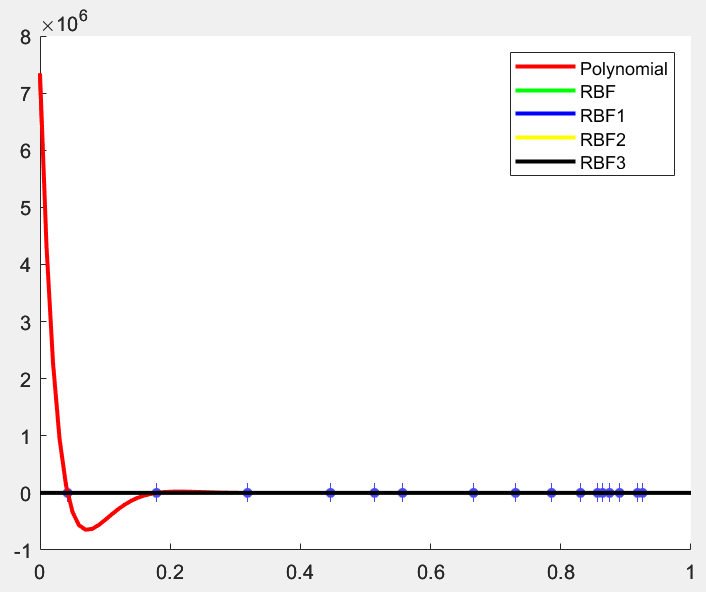
\includegraphics[scale=1]{result}%[width=0.7\linewidth, height=\textheight]
	\caption{}
	\label{fig:result0}
\end{figure}
\begin{figure}[H]
	\centering
	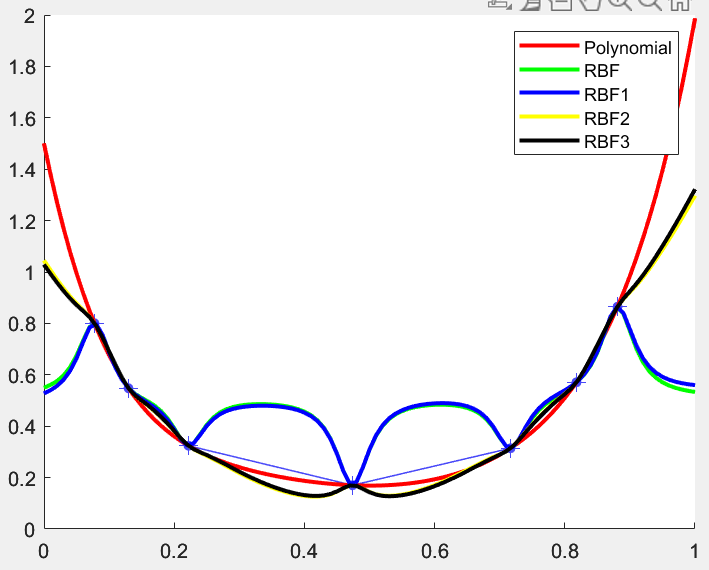
\includegraphics[scale=1]{result0}%[width=0.7\linewidth, height=\textheight]
	\caption{}
	\label{fig:result1}
\end{figure}
\begin{figure}[H]
	\centering
	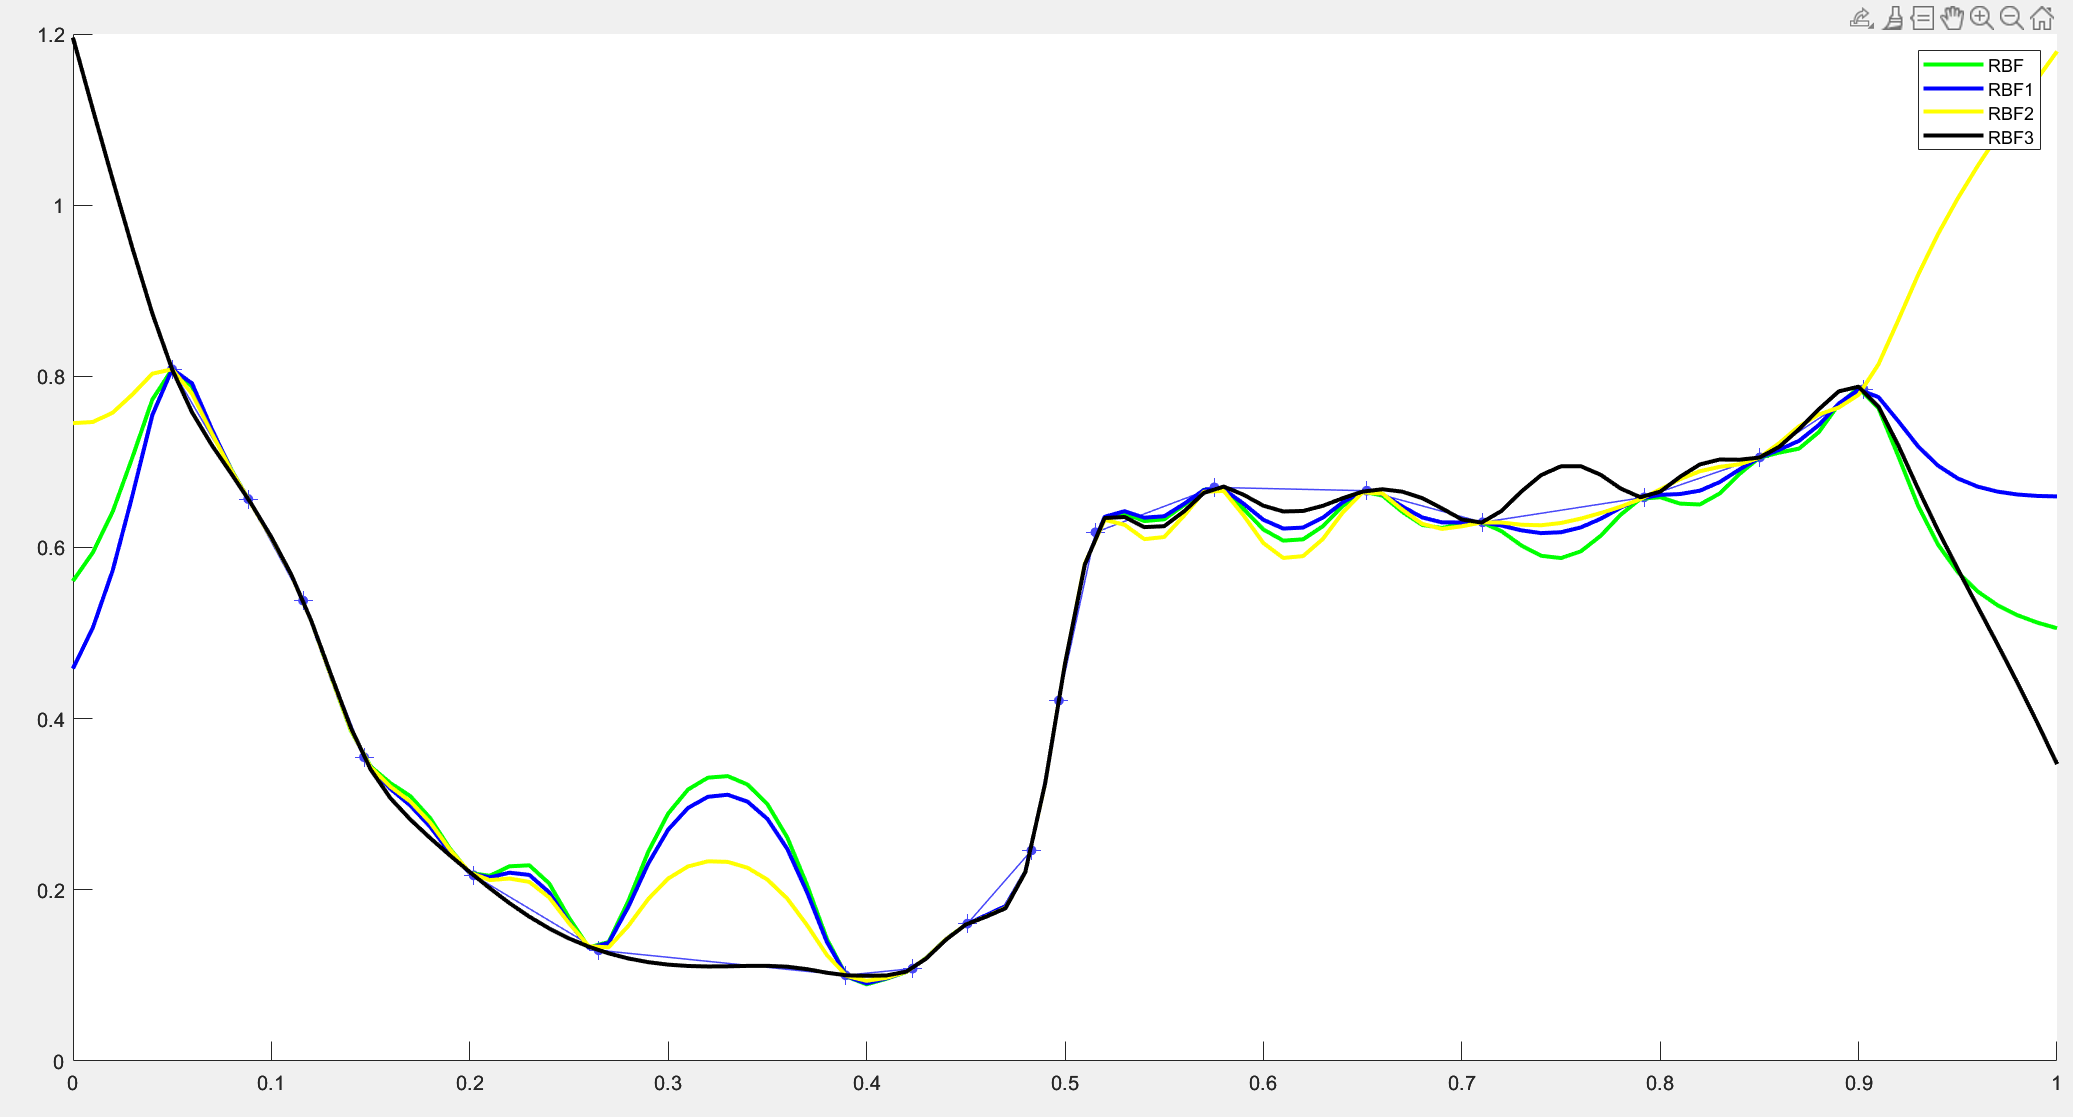
\includegraphics[scale=0.4]{result1}%[width=0.7\linewidth, height=\textheight]
	\caption{}
	\label{fig:result1}
\end{figure}


	\section{实验结果分析}
	多项式插值:在数据点较少且分布均匀时效果很好,但当数据点增多或分布不均时,可能会出现Runge现象,即多项式在区间边缘出现剧烈振荡。适用于数据点较少且分布均匀的情况,或者当需要一个简单、低阶的插值多项式时。
	
	RBF插值:通常能够提供更平滑的插值曲面,并且对于数据点的分布不敏感,因此在处理散乱数据时更为稳健。适用于数据点数量较多、分布不均匀或者需要高度平滑插值曲面的情况。对于本次实验中的$b_0(x)$,次数越高拟合效果越好。
\end{document}